\documentclass[11pt,a4paper]{article}
\usepackage[T1]{fontenc}\usepackage[utf8]{inputenc}
\usepackage{lmodern,microtype,amsmath,amssymb,amsthm,mathtools}
\usepackage{booktabs,longtable,array,enumitem,xcolor,geometry,fancyhdr,hyperref,graphicx}
\geometry{margin=22mm}
\hypersetup{colorlinks=true,linkcolor=blue!55!black,urlcolor=blue,citecolor=blue!55!black,
 pdftitle={FIN ST1632--ST1721: Lindblad Sensitivity, Kernel Parameter Boxes, KKT Geometry, Symmetric Decisions and the q-Clock No-Go},
 pdfauthor={Krzysztof Żuchowski}}
\pagestyle{fancy}\fancyhf{}\fancyhead[L]{FIN ST1632--ST1721}\fancyhead[R]{Release 11.02}\fancyfoot[C]{\thepage}\setlength{\headheight}{14pt}
\newtheorem{theorem}{Theorem}\newcommand{\status}[1]{\textsf{[#1]}}

\begin{document}
\begin{titlepage}\centering\vspace*{14mm}
{\Huge\bfseries FIN ST1632--ST1721\par}\vspace{4mm}
{\LARGE Lindblad Sensitivity, Kernel Parameter Boxes,\par}\vspace{2mm}
{\LARGE KKT Geometry, Symmetric Decisions and the $q$--Clock No-Go\par}\vspace{12mm}
{\Large Krzysztof \.Zuchowski\par}
{\normalsize Independent Researcher --- Fractal Information Theory Project\par}
{\normalsize ORCID: 0009-0002-0909-3613\par}\vspace{9mm}
{\large Six research rounds --- 90 programmes\par}
{\large Release 11.02 --- 31 August 2026\par}
\vfill
\begin{minipage}{.87\textwidth}\small
This report extends the conditional FIN discriminator from propagator
perturbations to the declared dephasing Lindbladian, propagates explicit kernel
parameter boxes, isolates the reduced continuous-minimax KKT candidate,
constructs a symmetric finite-grid decision with abstention, certifies a
vertex-detector matrix ball, and proves that fine-fiber $q$ and clock scale
cannot be identified separately without an anchor.
\end{minipage}\vfill
{\small English mathematical and computational research report.}
\end{titlepage}

\begin{abstract}
ST1632--ST1721 advance the conditional Operational/State programme at the
generator, parameter, inference and calibration levels.

For the declared energy-dephasing generator
\[
\mathcal L_A=-i\,\mathrm{ad}_A-\frac{\gamma}{2}\mathrm{ad}_A^2,
\]
self-adjoint graph perturbations $\|B-A\|\le\epsilon$ satisfy
\[
\|\mathcal L_B-\mathcal L_A\|
\le2\epsilon+2\gamma\epsilon(\|A\|+\|B\|).
\]
Each semigroup is Hilbert--Schmidt contractive, so Duhamel's formula propagates
this bound to return probabilities.  For $\gamma\le100$ and
$\epsilon=8.0418727748\times10^{-8}$, the certified four-time residual lower
bound remains $0.10789050485132269$.  The theorem is specific to the jump
operator $A$ and does not cover arbitrary GKSL operators.

The strict kernel parameter map
\[
w_d=\frac{\cos(\omega d+\phi)}{1+\beta d^\eta}
\]
is propagated by outward intervals.  A diagnostic large box with radii
$(5\times10^{-6},5\times10^{-6},5\times10^{-5},5\times10^{-5})$ gives
$\|\Delta A\|\le2.0105649071\times10^{-4}$: it preserves the simple
$t=0.6$ channel gap but fails the existing optimum/composite sufficient gates.
A small box with radii
$(2\times10^{-9},2\times10^{-9},2\times10^{-8},2\times10^{-8})$ gives
$\|\Delta A\|\le8.0418727748\times10^{-8}$ and passes.  Neither box is a
measured or strict confidence interval.

The reduced continuous minimax KKT geometry is isolated strongly numerically.
The candidate lies on the clock boundary $\alpha=1.1$, with
\[
\gamma_*\approx16.0591725623,qquad
w\approx(0.3185956783,0.6814043217),
\]
and value $0.053705210722682$, inside the certified continuous bracket
$[0.05,0.05370588868619479]$.  Equal endpoint divergences and the nuisance
stationarity equation are satisfied numerically; exact KKT isolation and a
global active-set theorem remain open.

For the finite nuisance grid, a symmetric decision with abstention is proved.
The mixture-likelihood boundary rejects the classical model, while the
condition that every component likelihood is below $0.01$ rejects the entire
grid in favour of the classical model.  Either wrong boundary has probability
at most one percent under its declared null, and the boundaries are mutually
exclusive.  Off-grid quantum models are not covered.

An arbitrary column-stochastic vertex detector with at most five percent
misclassification per true vertex changes any distribution by at most five
percent in total variation.  Independent classical/quantum detectors therefore
leave simple-model TV at least $0.3112182255$.

Finally, physical-time fine-fiber returns depend only on
\[
\kappa=\frac{q}{\tau_*}.
\]
The transformation $(q,\tau_*)\mapsto(cq,c\tau_*)$ leaves every number of heat
and unitary fiber observations invariant.  Thus $q$ and the clock scale are
not jointly identifiable without an independent anchor.  Protocol 11.02
freezes these conclusions; no apparatus or physical calibration is supplied.
\end{abstract}

\tableofcontents\newpage

\section{Round I: ST1632--ST1646 --- Lindblad sensitivity}

On Hilbert--Schmidt operator space define
\[
\mathrm{ad}_A(X)=AX-XA,qquad
\mathcal L_A=-i\mathrm{ad}_A-\frac{\gamma}{2}\mathrm{ad}_A^2.
\]
For $E=B-A$,
\[
\|\mathrm{ad}_B-\mathrm{ad}_A\|\le2\|E\|=2\epsilon.
\]
Using
\[
X^2-Y^2=(X-Y)X+Y(X-Y)
\]
and $\|\mathrm{ad}_A\|\le2\|A\|$ gives
\[
\|\mathrm{ad}_B^2-\mathrm{ad}_A^2\|
\le4\epsilon(\|A\|+\|B\|),
\]
and hence
\[
\Delta_{\mathcal L}equiv\|\mathcal L_B-\mathcal L_A\|
\le2\epsilon+2\gamma\epsilon(\|A\|+\|B\|).
\]

For self-adjoint $A$, $\mathcal L_A$ is a normal dissipative function of
$\mathrm{ad}_A$; $e^{t\mathcal L_A}$ is Hilbert--Schmidt contractive.  Thus
\[
\|e^{t\mathcal L_B}-e^{t\mathcal L_A}\|
\le t\Delta_{\mathcal L}.
\]
Rank-one state/effect Hilbert--Schmidt norms are one, so the same upper bound
controls the measured return.

With $\|A\|=2.3421820411463$, $\gamma=100$, $t\le2$ and
$\epsilon=8.041872774817993\times10^{-8}$, the dephased-quantum plus heat-
target perturbation is at most $1.5116675487625433\times10^{-4}$.  Subtracting
it from $0.10804167160619894$ yields
\[
0.10789050485132269>0.
\]

\begin{theorem}[declared dephasing robustness]
The four-time composite separation remains positive under the stated small
noncirculant graph perturbation for every $0\le\gamma\le100$.
\end{theorem}

This theorem does not cover independent or non-$A$ jump operators, trace-norm
contraction claims, or non-Markov heat.

\section{Round II: ST1647--ST1661 --- kernel parameter boxes}

The nominal parameter tuple is
\[
(\omega,\phi,\beta,\eta)=(0.18575,0.16250,1,1.8).
\]
Outward interval evaluation of all six distances constructs weight intervals,
the row-sum diagonal and a circulant row-norm bound for $\Delta A$.

\paragraph{Large diagnostic box.}
Radii
\[
(5\times10^{-6},5\times10^{-6},5\times10^{-5},5\times10^{-5})
\]
give
\[
\|\Delta A\|\le0.00020105649070913632.
\]
Every weight stays positive, and the simple return gap remains above $0.41085$
by Duhamel.  However this box is wider than the global-location threshold and
the present $\gamma=100$ composite sufficient bound.  This is failure to
certify, not a counterexample.

\paragraph{Small certified box.}
Radii
\[
(2\times10^{-9},2\times10^{-9},2\times10^{-8},2\times10^{-8})
\]
give
\[
\|\Delta A\|\le8.041872774817993\times10^{-8},
\]
which passes both the location and declared Lindblad-composite gates.

The interval map is conservative because the same parameters occur at every
distance and in the diagonal, while elementary interval evaluation loses some
correlation.  More importantly, neither box has repository or experimental
confidence-level provenance.  The small box is a mathematical witness, not a
physical error bar.

\section{Round III: ST1662--ST1676 --- reduced KKT candidate}

The continuous minimax certificate from Release 11.01 bounds the value but not
the optimizing weights.  The numerical LP suggests a two-time face at
$t_1=0.3$, $t_2=2.0$ and clock boundary $\alpha=1.1$.

Near the candidate, the active divergence at each time is
$D(C_i\|Q_i)$.  An interior allocation requires equality of the two active
endpoint divergences:
\[
d_{0.3}(\gamma)=d_{2.0}(\gamma).
\]
Brent isolation gives
\[
\gamma_*\approx16.05917256231611.
\]
The nuisance-stationarity condition
\[
w d'_{0.3}(\gamma_*)+(1-w)d'_{2.0}(\gamma_*)=0
\]
then gives
\[
w\approx0.31859567830451857,qquad1-w\approx0.6814043216954815.
\]
The common active value is
\[
0.053705210722682,
\]
consistent with the certified global bracket.

The one-sided derivative in $\alpha$ is consistent with a minimum at the upper
clock boundary, and middle times have positive reduced costs in the fine LP.
These are strong numerical KKT checks.  No interval Jacobian, exact root or
global active-set theorem is claimed.

\section{Round IV: ST1677--ST1691 --- symmetric grid decision}

Let $L_{j,n}$ be the likelihood ratio for grid component $j$, and let
\[
E_n=\sum_j\pi_jL_{j,n}.
\]
The decision set is
\begin{align*}
E_n\ge100 &\quad\Rightarrow\quad Q_{\rm mixture},\\
\max_jL_{j,n}\le0.01 &\quad\Rightarrow\quad C_{\rm all-grid},\\
\text{otherwise} &\quad\Rightarrow\quad \text{continue/abstain}.
\end{align*}

Under $C$, $E_n$ is an e-process, so a false quantum boundary has probability
at most $0.01$.  If grid component $j_0$ is true, the event
$\max_jL_{j,n}\le0.01$ implies $1/L_{j_0,n}\ge100$; Ville's inequality bounds
a false classical boundary by $0.01$.  The boundaries are mutually exclusive:
if every $L_j\le0.01$, their convex mixture cannot exceed $0.01$.

\begin{theorem}[finite-grid symmetric decision]
The three-decision rule has one-percent anytime wrong-boundary control under
the classical model and under every frozen grid quantum model, with abstention
allowed.
\end{theorem}

Synthetic fixtures reached the classical and quantum boundaries after 142 and
a model-dependent number of events.  They test code only.  Off-grid quantum
models have no uniform classical-boundary guarantee.  A formal continuum rule
would replace the maximum by $\sup_\theta L_{\theta,n}$ and the mixture by an
exact integral; its executable certification remains open.

\section{Round V: ST1692--ST1706 --- detector matrix and $q$--clock}

\subsection{Vertex detector ball}

Let $M$ be column stochastic and suppose every true vertex is reported
correctly with probability at least $1-\delta$.  Coupling each column with the
identity gives
\[
\operatorname{TV}(Mp,p)\le\delta.
\]
For independent detector matrices,
\[
\operatorname{TV}(M_Cp,M_Qq)
\ge\operatorname{TV}(p,q)-2\delta.
\]
At $t=0.6$, the ideal full-distribution TV is $0.4112182254653598$.  For
$\delta=0.05$,
\[
\operatorname{TV}_{\rm observed}\ge0.3112182254653598.
\]
The sufficient identifiability threshold is
$\delta<0.2056091127326799$.  A common matrix may admit sharper Dobrushin or
inverse-calibration bounds, but the triangle bound remains valid.

Loss can be represented as a thirteenth no-click outcome, restoring a
column-stochastic augmented detector.  Discarding it reintroduces
postselection blindness.

\subsection{Joint $q$--clock obstruction}

With physical time, the fine returns are
\[
H(t_{\rm phys})=\frac{1+\exp[-2q\,t_{\rm phys}/\tau_*]}{2},
\qquad
R(t_{\rm phys})=\cos^2(q\,t_{\rm phys}/\tau_*).
\]
Every record depends only on
\[
\kappa=\frac{q}{\tau_*}.
\]

\begin{theorem}[joint $q$--clock no-go]
The transformation
\[
(q,\tau_*)\mapsto(cq,c\tau_*),\qquad c>0,
\]
leaves all fine heat and unitary return probabilities invariant at every
physical time.  No number of such observations identifies $q$ and $\tau_*$
separately.
\end{theorem}

An independent calibration of $\tau_*$ restores the earlier conditional
$q$-identifiability results.  Multiple scheduled times alone do not.

\begin{figure}[ht]
\centering
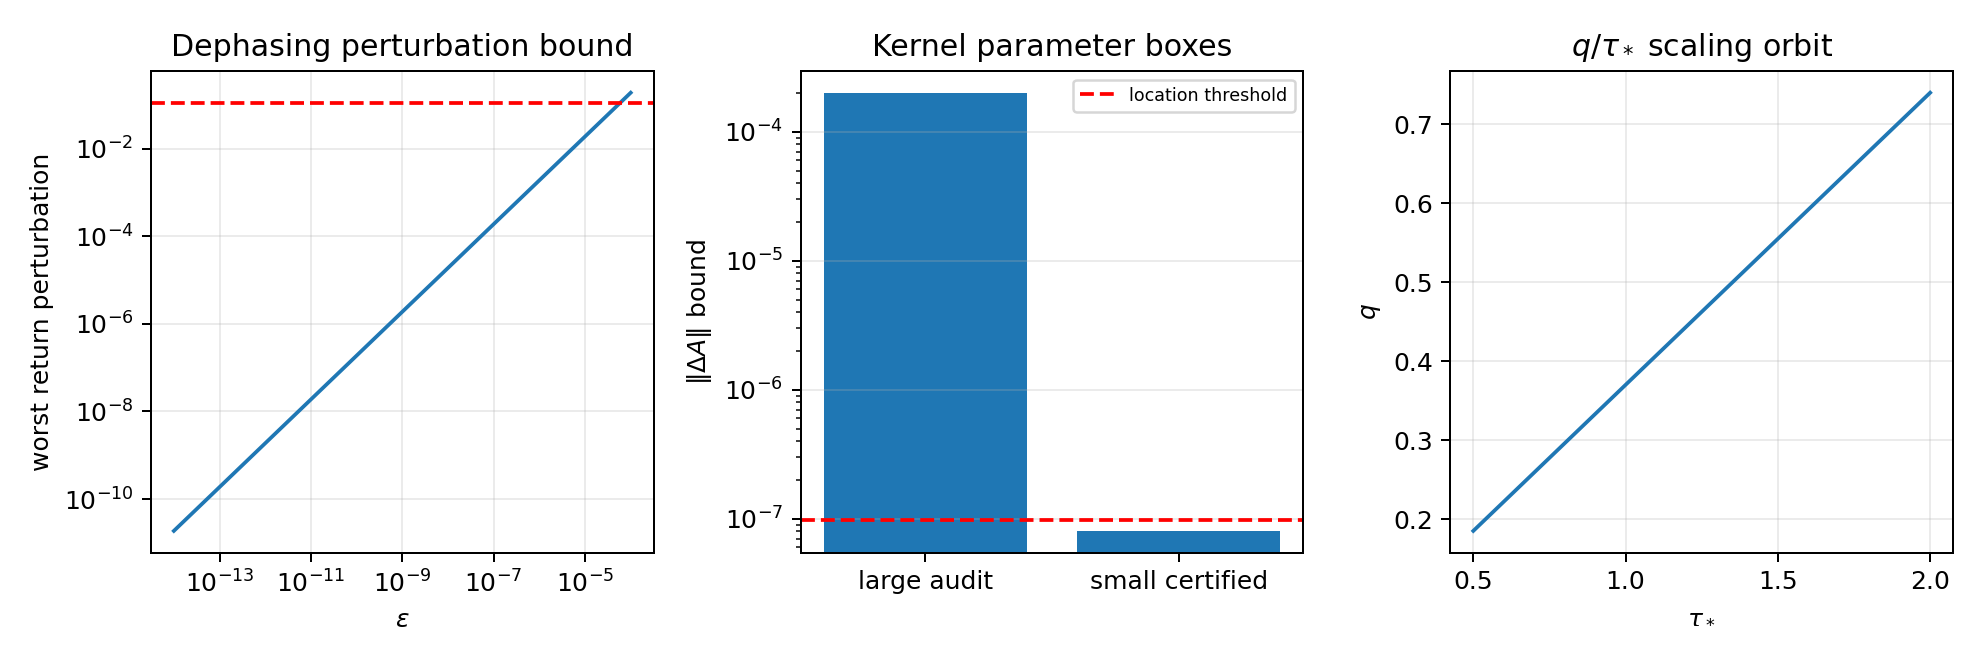
\includegraphics[width=.98\textwidth]{FIN_ST1632_ST1721_Figures/lindblad_kernel_qclock_summary.png}
\caption{Left: declared dephasing perturbation bound.  Centre: large and small
kernel-parameter boxes relative to the location threshold.  Right: the exact
$q/\tau_*$ scaling orbit.}
\end{figure}

\section{Round VI: ST1707--ST1721 --- synthesis}

\begin{longtable}{@{}p{.34\textwidth}p{.22\textwidth}p{.34\textwidth}@{}}
\toprule
Result & Status & Boundary \\
\midrule\endhead
declared Lindblad sensitivity & \status{Proven} & jump operator $A$, HS norm \\
large parameter box & \status{Partial} & base gap only \\
small parameter box & \status{Interval-proven} & no physical CI provenance \\
continuous minimax value & \status{Certified bracket} & exact weights open \\
reduced KKT geometry & \status{Strong numerical} & active-set theorem open \\
symmetric grid decision & \status{Proven} & finite grid, abstention \\
vertex detector TV ball & \status{Proven} & column-error class \\
joint $q$--clock identification & \status{Refuted} & exact scaling torsor \\
platform/evidence & \status{Absent} & no calibrated device/events \\
\bottomrule
\end{longtable}

Protocol \path{FIN_ST1707_ST1721_Protocol_11_02.json} hashes Release 11.01,
the continuous-prior object, independent calibration and the detector/$q$--clock
artifact, and records the Lindblad bound, kernel boxes, KKT candidate and
symmetric decision.

These results strengthen a conditional $OA$ only.  They do not derive the
state category, parameter uncertainty, clock anchor or apparatus from strict
FIN.

The tests concern internal channel and parameter inference, not literal
annihilation of the whole nadsoliton.

\section{Recommended next programmes}

\begin{enumerate}
\item certify a general GKSL jump-operator ball;
\item derive a parameter interval from strict kernel provenance;
\item isolate the KKT root with interval Newton/Krawczyk methods;
\item certify the continuum supremum-likelihood boundary;
\item combine detector confusion and loss in one augmented matrix polytope;
\item add a second observable with a different $q/\tau$ scaling weight;
\item impose multi-fiber $q$ consistency;
\item optimize a continuous prior for power while preserving validity;
\item derive a platform-specific forward model;
\item freeze external clock calibration;
\item obtain independent audit;
\item collect raw events only after every freeze.
\end{enumerate}

Stop if the $A$-dephasing bound is used for arbitrary jumps, the small box is
called a measured confidence interval, the KKT candidate is called the exact
optimizer, the finite grid is called a continuum decision, the TV ball is
called a calibrated apparatus, or $\kappa$ is called separate knowledge of
$q$ and $\tau_*$. 

\section{Final conclusion}

\begin{quote}
The conditional FIN discriminator now has theorem-level control at the
declared Lindblad-generator and detector-matrix levels, a certified continuous
minimax value, and symmetric finite-grid decisions with abstention.  The
fine-fiber analysis simultaneously reveals an exact scale torsor: internal
returns identify only $q/\tau_*$.  The next decisive bridge is therefore not
more curve fitting, but an independently sourced clock/scale observable and a
platform-calibrated operator family.
\end{quote}

\appendix
\section{Six-round ledger}
\begin{longtable}{@{}p{.18\textwidth}p{.34\textwidth}p{.38\textwidth}@{}}
\toprule
Range & Object & Verdict \\
\midrule\endhead
ST1632--ST1646 & dephasing Lindbladian & noncirculant sensitivity bound \\
ST1647--ST1661 & kernel parameter boxes & large partial / small certified \\
ST1662--ST1676 & reduced KKT system & strong numerical candidate \\
ST1677--ST1691 & symmetric finite-grid decision & two boundaries plus abstention \\
ST1692--ST1706 & detector and $q$--clock & TV robustness and exact scale no-go \\
ST1707--ST1721 & synthesis & generator-to-inference robustness lattice \\
\bottomrule
\end{longtable}

\section{Reproducibility}
The authoritative result sets run from
\path{FIN_ST1632_ST1646_Results.json} through
\path{FIN_ST1707_ST1721_Results.json}.  Each contains fifteen programmes and
packet SHA-256 references.  The combined test
\path{test_fin_st1632_st1721.py} verifies all ninety packets, Lindblad bounds,
parameter gates, KKT status, symmetric decision, detector TV, $q$--clock
obstruction, protocol, figure and nonpromotion gates.

\section{Nonclaims}
No arbitrary GKSL uncertainty theorem, physical parameter confidence interval,
exact minimax optimizer, continuum symmetric decision, calibrated detector,
separate $q$/$\tau_*$ source, state ontology, platform, raw event, independent
custody, legacy bridge, selector, Standard Model, gravity, $L_{\rm total}$ or
Theory of Everything is established.  All future FIN PDFs remain English.

\begin{thebibliography}{9}
\bibitem{breuer} H.-P. Breuer and F. Petruccione, \emph{The Theory of Open Quantum Systems}, Oxford University Press.
\bibitem{engel} K.-J. Engel and R. Nagel, \emph{One-Parameter Semigroups for Linear Evolution Equations}, Springer.
\bibitem{ville} J. Ville, \emph{Etude critique de la notion de collectif}, Gauthier-Villars.
\end{thebibliography}
\end{document}
